\documentclass{article}
\usepackage{amsmath, fullpage}

%This command makes the font san serif
%which is best practice for readability.
\renewcommand{\familydefault}{\sfdefault}

% Load the setspace package
\usepackage{setspace}
% Using \doublespacing in the preamble 
% changes the text to double-line spacing
\doublespacing

%Load the package for hyper links
\usepackage{hyperref}
%%this ensures that the \url{} links are distinguished
%%by color
\hypersetup{colorlinks=true, urlcolor=cyan}

%Load the package for including pics
\usepackage{graphicx,float,caption}

\begin{document}

\title{Your Title Goes Here}
\author{Your Name Goes Here}
\date{\today}
\maketitle
\thispagestyle{empty}

\section{Introduction}\label{intro}

You may choose to toggle-off the double-spacing for yourself, but the pdf that you submit to me needs to be double spaced! 

Observe that the date updates automatically to the date on which the document was compiled.

Below is some math stuff. Recall that one uses dollar signs to typeset mathematics. 

A sequence $(X_1, Y_1), (X_2,Y_2),\ldots, (X_n, Y_n)$ and an equation $y = a + bx.$ Next is an expression \emph{not} in displaystyle 
$E = \sum_{i=1}^n (Y_i - a - bX_i)^2,$ followed by the same expression \emph{in} displaystyle $\displaystyle{E = \sum_{i=1}^n (Y_i - a - bX_i)^2}.$

Last, we show the use of double-dollar-signs to both center and use displaystyle formatting. This includes the use of spacers (\textbackslash quad) and the \textbackslash text command to get precise formatting.
$$
x_i = \frac{X_i - \overline{X}}{\sqrt{\sum (X_i - \overline{X})^2}}\quad\text{and}\quad
y_i = \frac{Y_i - \overline{Y}}{\sqrt{\sum (Y_i - \overline{Y})^2}}.
$$

For long strings of equations you would like to align, see the example below.
\begin{align*}
E &= \sum (y_i - a - bx_i)^2 \\
&= \sum (y_i^2 + a^2 + b^2 x_i^2 - 2ay_i - 2bx_iy_i + 2abx_i) \\
&= \sum y_i^2 + \sum a^2 + \sum b^2 x_i^2 
 - \sum 2ay_i - \sum 2bx_iy_i + \sum 2abx_i \\
&= 1 + na^2 + b^2 - 2br \\
&= (1-r^2) + na^2 + (b - r)^2\ .
\end{align*}

For a pair of equations to align at the equal sign, one on top of the other, see the example below. Note the use of ``\textbackslash left (" to force parentheses to be the right size.

\begin{align*}
\frac{y - \overline{Y}}{\sqrt{\sum (Y_i - \overline{Y})^2}}
&= \left(
     \frac{\sum (X_i - \overline{X}) (Y_i - \overline{Y})}
          {\sqrt{\sum (X_i - \overline{X})^2 \sum (Y_i - \overline{Y})^2}}
   \right)
   \left(
     \frac{x - \overline{X}}
          {\sqrt{\sum (X_i - \overline{X})^2}}
   \right)\\
y - \overline{Y} &=
\left(
     \frac{\sum (X_i - \overline{X}) (Y_i - \overline{Y})}
          {\sum (X_i - \overline{X})^2}
   \right)
   (x - \overline{X})\ .
\end{align*}

In Section \ref{figures}, I will tell you about displaying images. In Section \ref{tables}, you will find examples of tables. I'm not sure you will need them but there ya go. In Section \ref{bib} you will find a template for manually including a bibliography. 

\section{Figures}\label{figures}

Below is a picture using the includegraphics command.

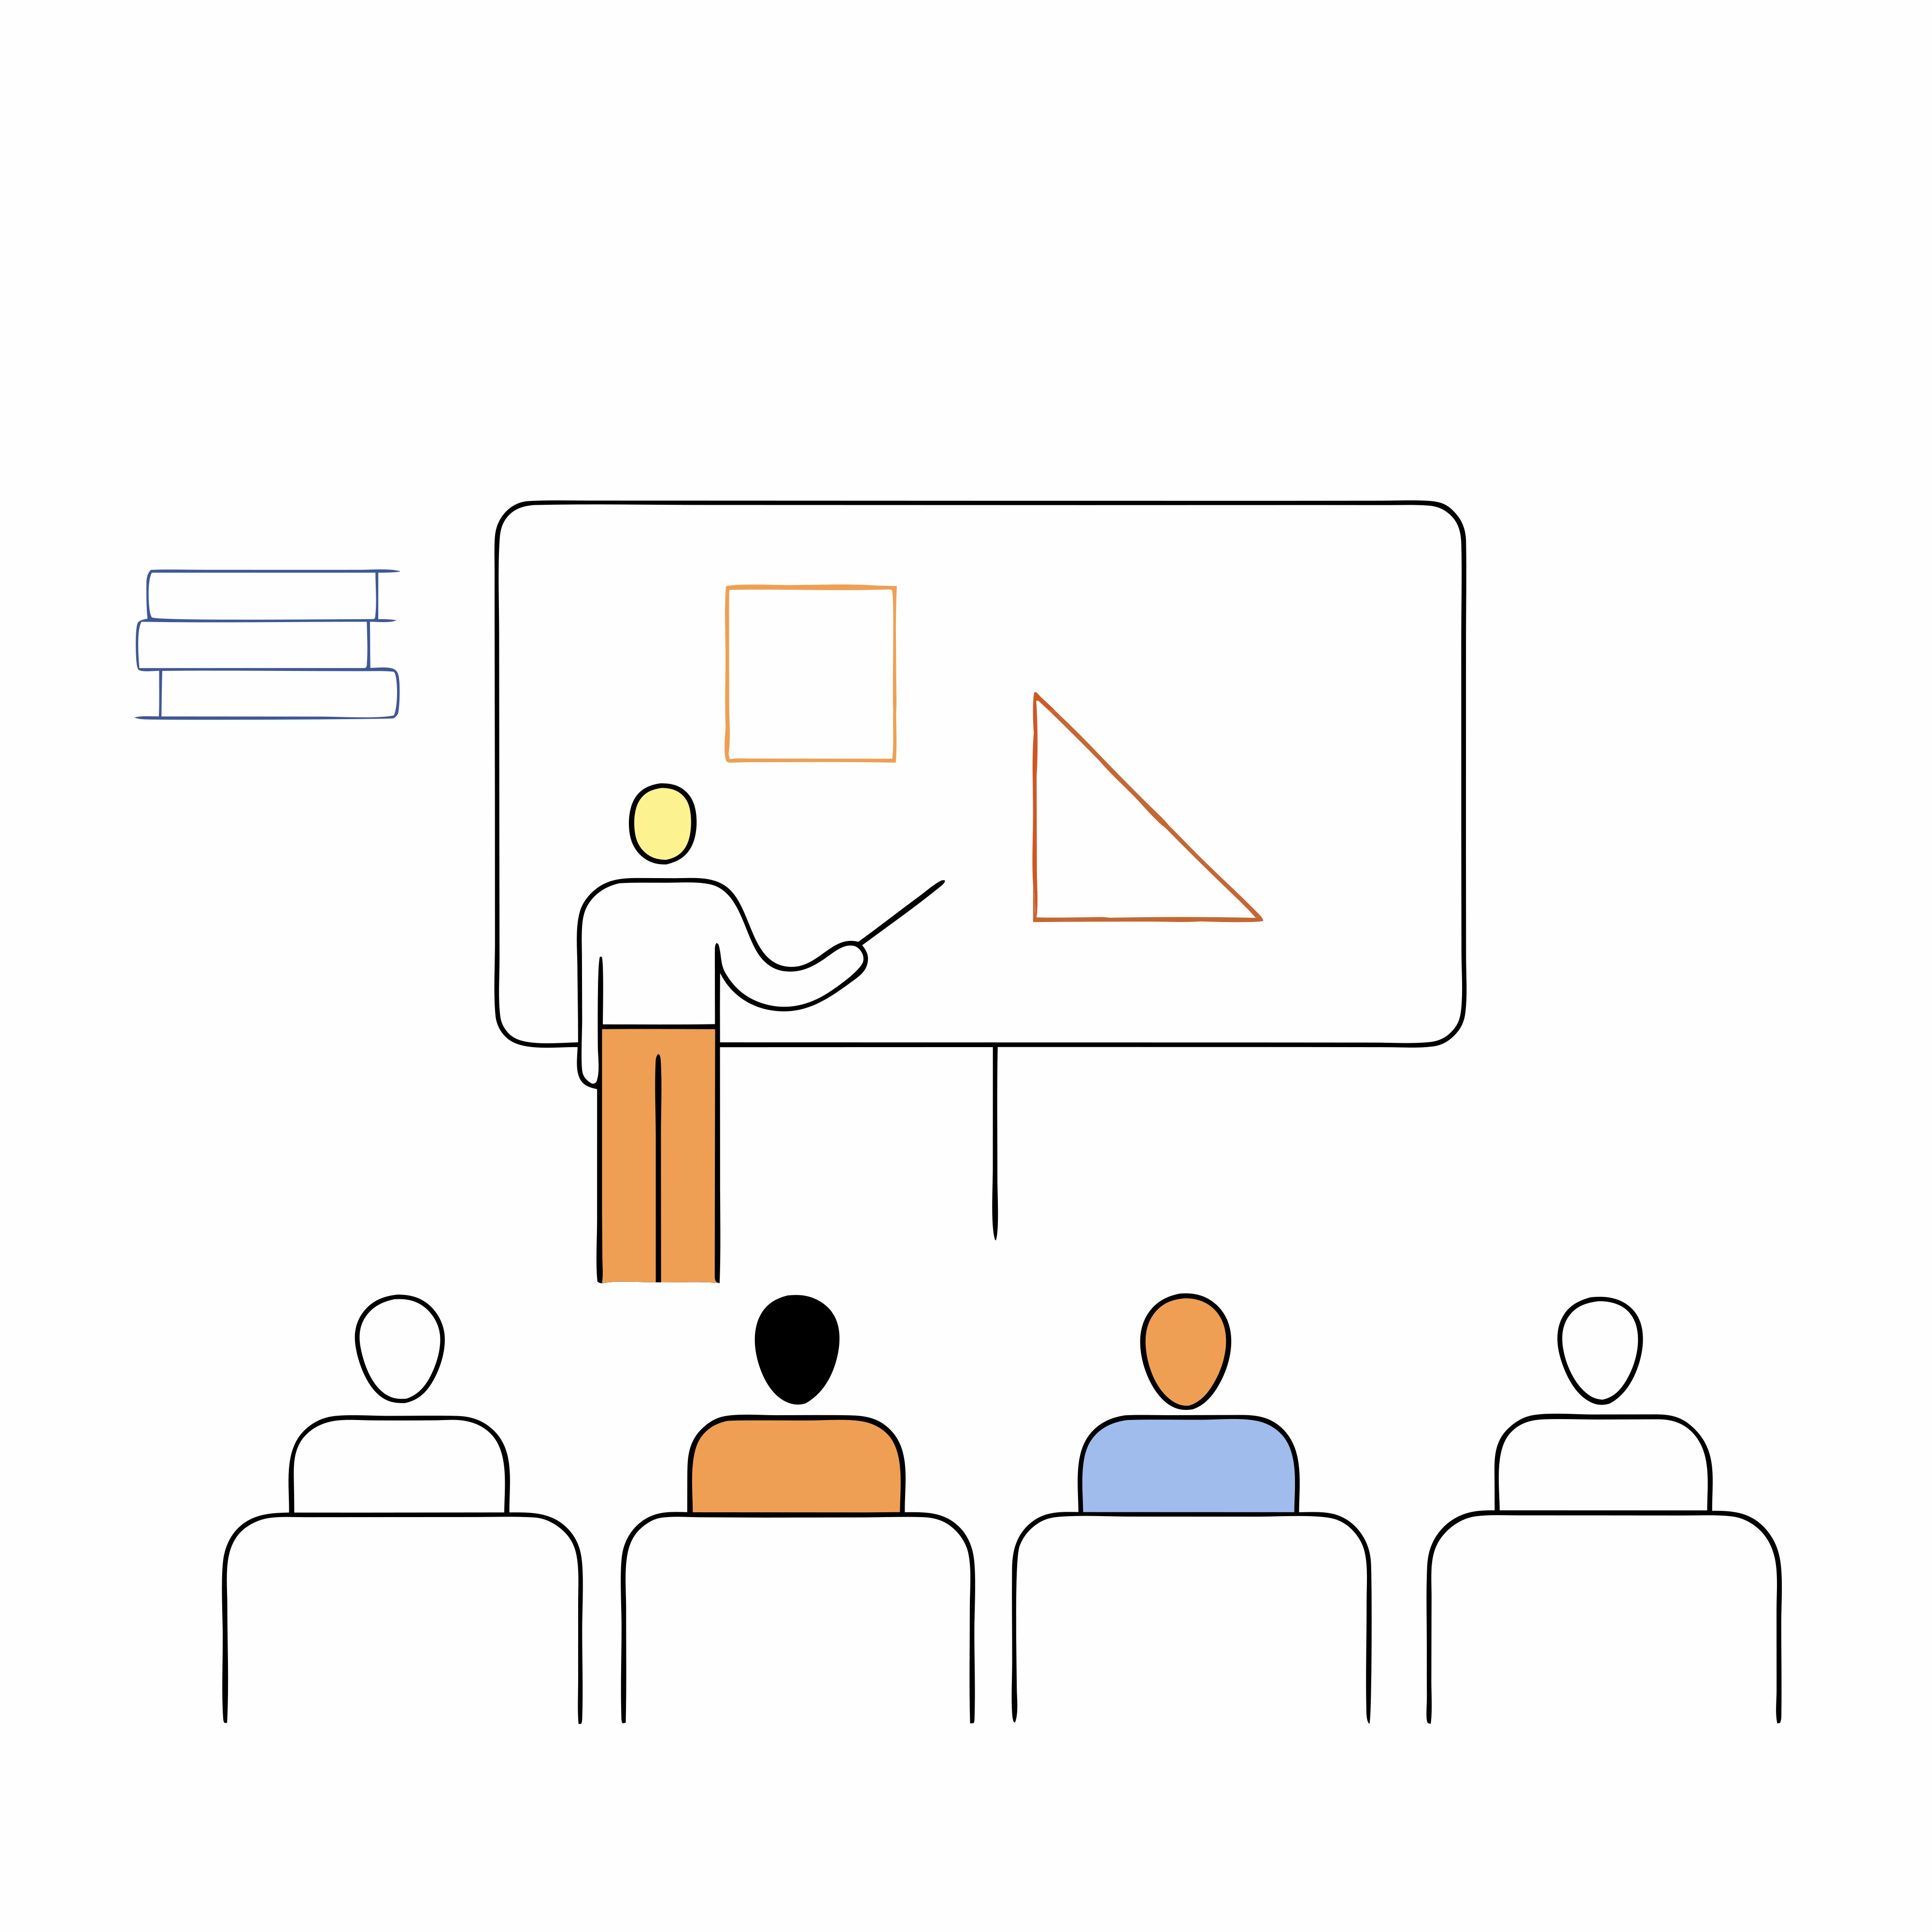
\includegraphics[scale=0.03]{momo.png}

In Figure \ref{man}, you will see the same picture but in the figure formatting so that it can be referenced and have a caption. You should include any pictures inside the figure structure for clarity.

\begin{figure}[H]
\centering
\captionsetup{width=.5\linewidth}
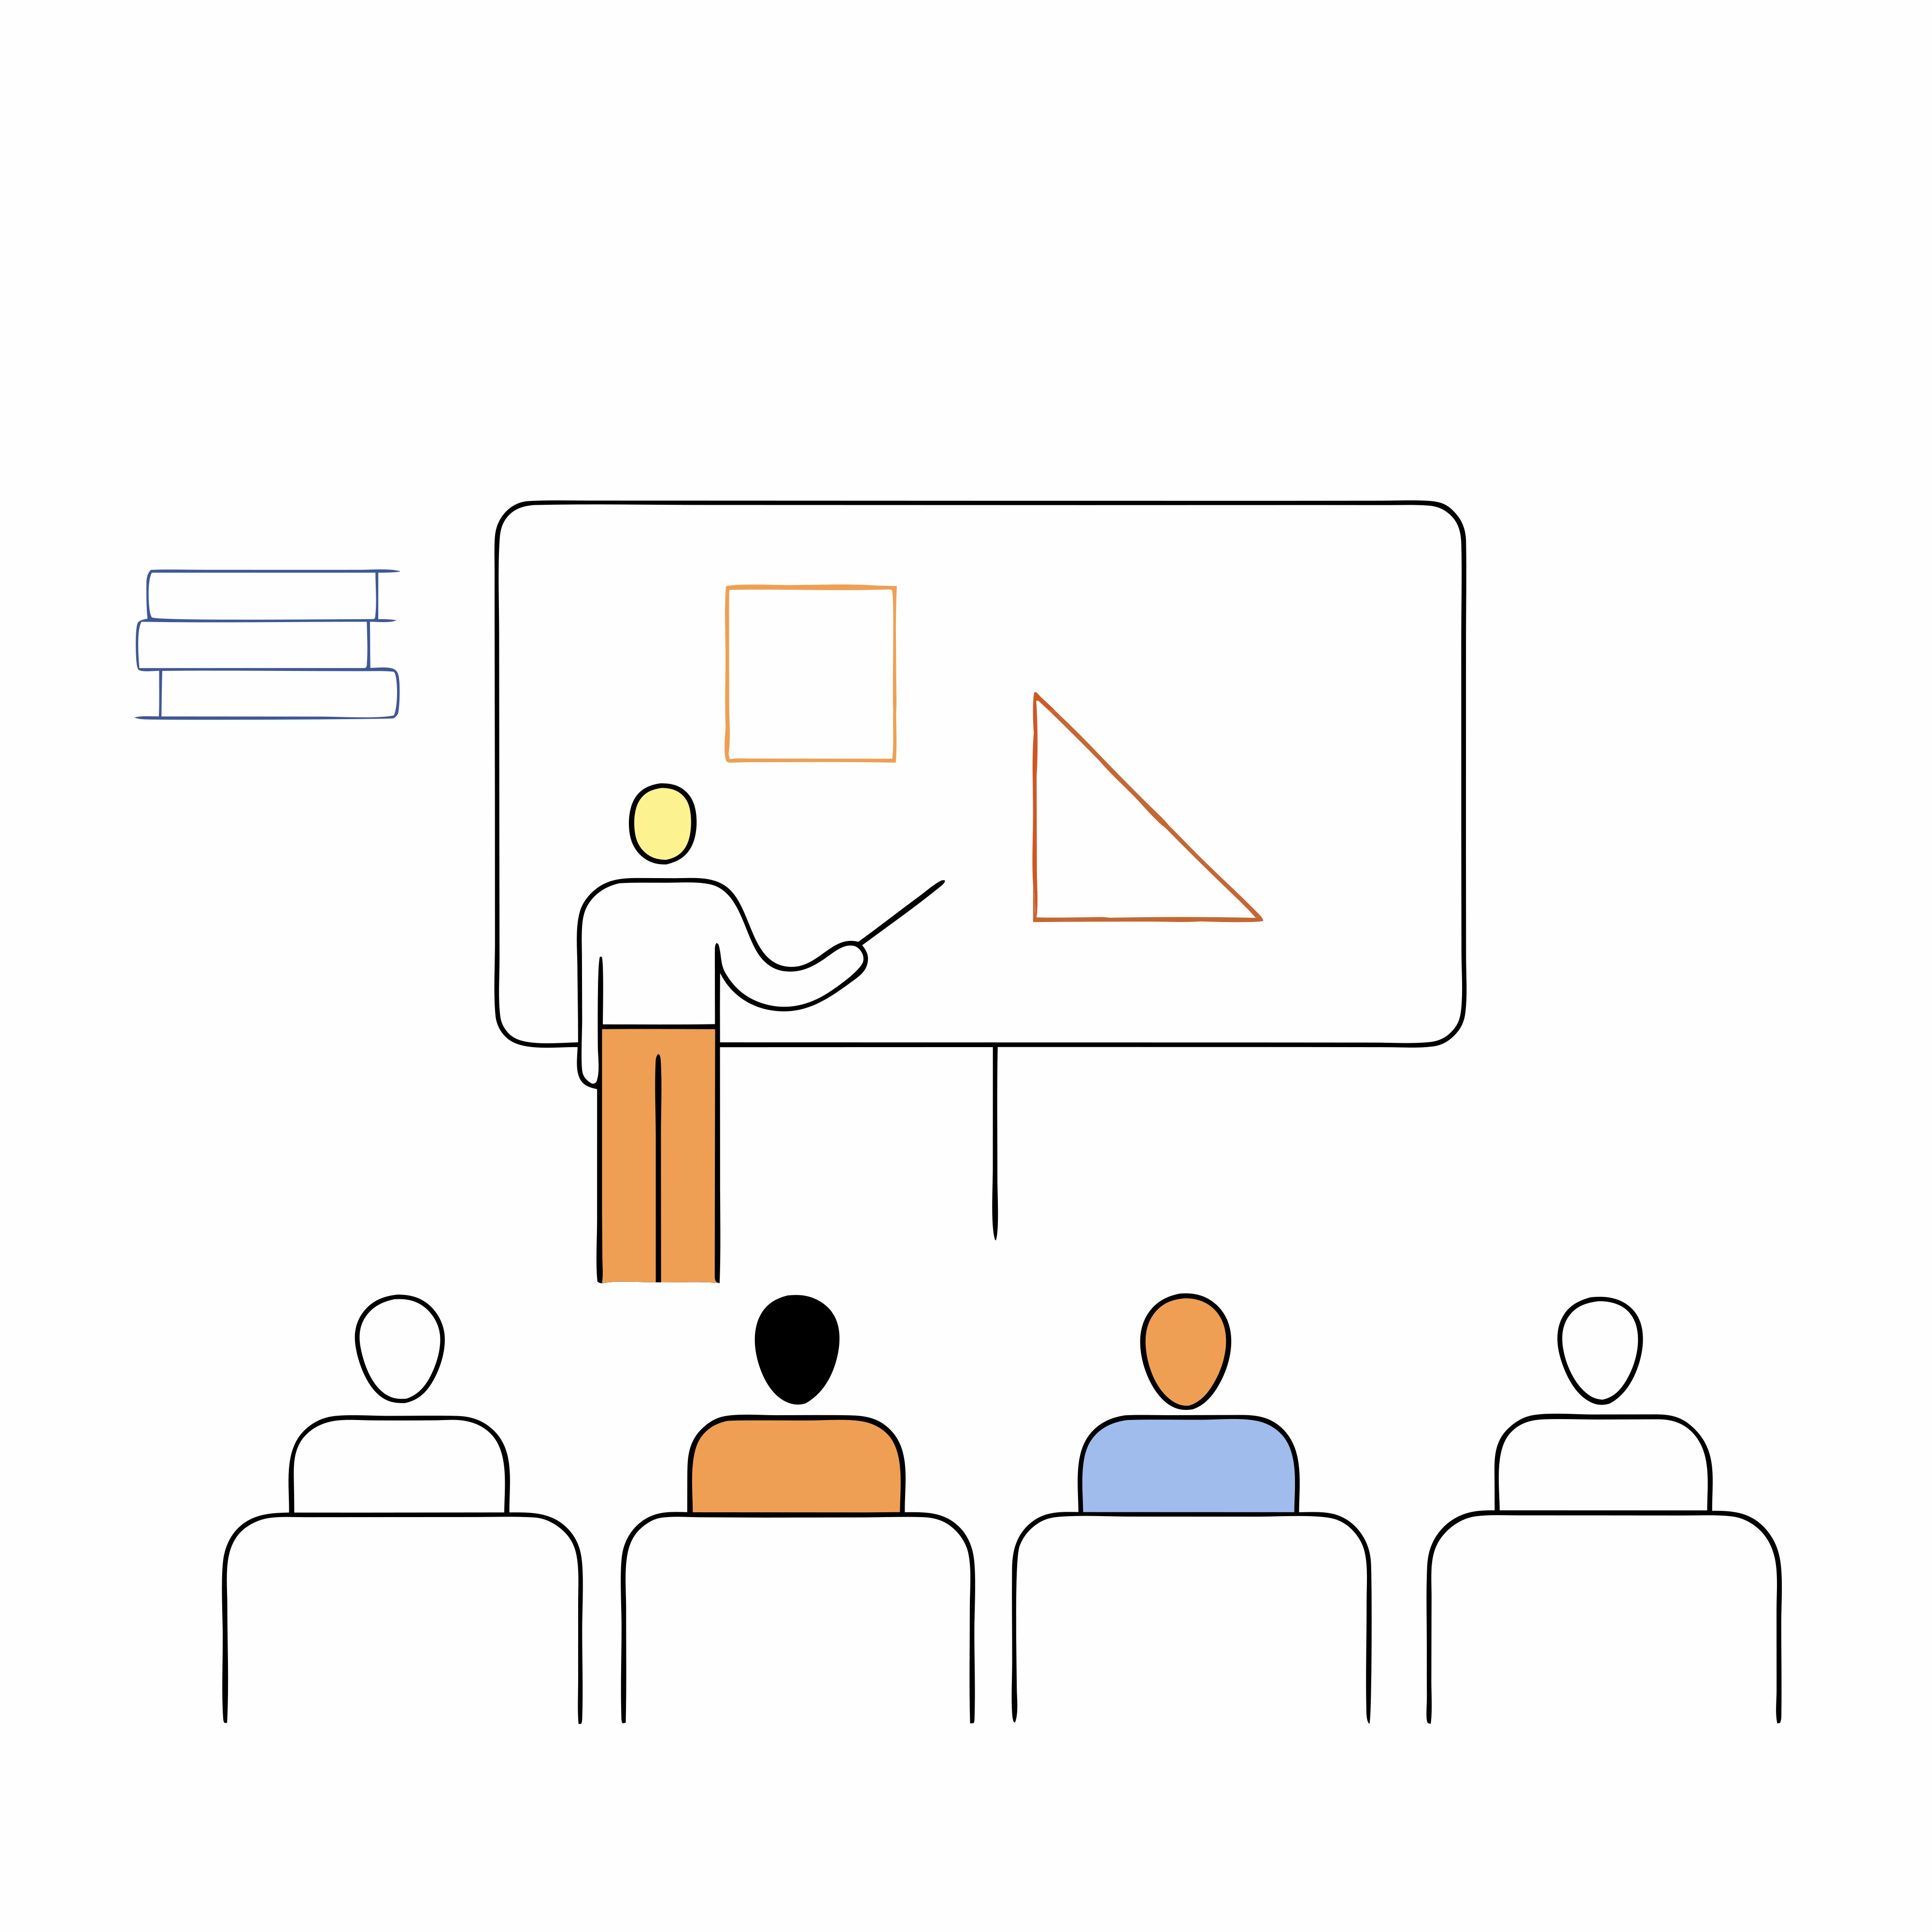
\includegraphics[scale=0.03]{momo.png}
\caption{This is a picture I retrieved from Unsplash by creator called Momo Studio \cite{momo} on March 2025}
\label{man}
\end{figure}

You will see another figure, centered, in Figure \ref{tungay}.

\begin{figure}
\centering
\captionsetup{width=.5\linewidth}

\includegraphics[scale=0.03]{tungay.jpg}
\caption{This is a picture I retrieved from Unsplash by creator called K. Tungay \cite{t25} on March 2025}
\label{tungay}
\end{figure}


Note that the source file for the figure needs to be in the same location as the \textit{filename.tex} file.



\section{Tables}\label{tables}

Here are some tables. 


\begin{tabular}{ c | c | p{1.5in}}
Explored? & vertices & tentative distances\\ \hline
&S& \\[12pt] \hline
&A& \\[12pt]\hline
&B& \\[12pt]\hline
&C& \\[12pt]\hline
&D& \\[12pt]\hline
&E& \\[12pt]\hline
 \end{tabular}
 \quad and \quad
 \begin{tabular}{ r | p{.8in} }
 vertex & minimum distance to S\\ \hline
S& \\[12pt] \hline
A& \\[12pt]\hline
B& \\[12pt]\hline
C& \\[12pt]\hline
D& \\[12pt]\hline
E& \\[12pt]\hline \end{tabular}
 
\vfill



\section{Bibliography}\label{bib}



For future reference, there are automated ways of managing a bibliography, but these require some additional files and can make compiling tricky. Thus, for this class, I suggest hand-coding it. 

There are to things to note. You can (and should) reference the sources in the body of your text. For example, maybe I cite the online version of the Euclid's Elements here \cite{elements} and the book is cited here \cite{our_text}.

Linking references or citations will require that you compile \emph{twice}. That is, after the \emph{first} compile, all references will be ??. On the second, you will get the proper number/citation.

\begin{thebibliography}{widest entry}
 \bibitem[Burton11]{our_text} Burton, David M. The History of Mathematics: An Introduction. 7th ed., McGraw-Hill, 2011. 
 \bibitem[Joyce98]{elements} Joyce, David E.. "Euclid's Elements, Introduction" Department of Mathematics and Computer Science, Clark University, 1998, \url{http://aleph0.clarku.edu/~djoyce/java/elements/elements.html}.
 
 \bibitem[MomoStudio]{momo} Momo Studio, Man Giving a Presentation [Illustration]. Unsplash. \url{https://unsplash.com/illustrations/a-man-giving-a-presentation-to-a-group-of-people-mvbZKEDrLuk}
 
 \bibitem[Tungay25]{t25} Tungay, K. Pile of Color Pencils [Photograph]. Unsplash. \url{https://unsplash.com/photos/pile-of-color-pencils-2LJ4rqK2qfU}.
 
% Smith, J. (2023). Sunset Over the Ocean [Photograph]. Pixabay. pixabay.com/photos/sunset-beach-landscape-3981724/.
% 
% Photo by <a href="https://unsplash.com/@kellitungay?utm_content=creditCopyText&utm_medium=referral&utm_source=unsplash">Kelli Tungay</a> on <a href="https://unsplash.com/photos/pile-of-color-pencils-2LJ4rqK2qfU?utm_content=creditCopyText&utm_medium=referral&utm_source=unsplash">Unsplash</a>
%      
% 
\end{thebibliography}



\end{document}
